        %%******************************************%%
        %%                                          %%
        %%        Modello di tesi di laurea         %%
        %%            di Andrea Giraldin            %%
        %%                                          %%
        %%             2 novembre 2012              %%
        %%                                          %%
        %%******************************************%%


% I seguenti commenti speciali impostano:
% 1. 
% 2. PDFLaTeX come motore di composizione;
% 3. tesi.tex come documento principale;
% 4. il controllo ortografico italiano per l'editor.

% !TEX encoding = UTF-8
% !TEX TS-program = pdflatex
% !TEX root = tesi.tex
% !TEX spellcheck = it-IT

% PDF/A filecontents
\RequirePackage{filecontents}
\begin{filecontents*}{\jobname.xmpdata}
  \Title{Studio e sviluppo di un web crawler intelligente per dark web e
surface web}
  \Author{Daniele Giachetto}
  \Language{it-IT}
  \Subject{Il presente documento descrive il lavoro svolto durante il periodo di stage dal laureando Daniele Giachetto presso l’azienda Yarix S.r.l..}
  \Keywords{Cyber security\sep Dark web\sep webcrawler}
\end{filecontents*}

\documentclass[10pt,                    % corpo del font principale
               a4paper,                 % carta A4
               twoside,                 % impagina per fronte-retro
               openright,               % inizio capitoli a destra
               english,                 
               italian,                 
               ]{book}    

%**************************************************************
% Importazione package
%************************************************************** 

\PassOptionsToPackage{dvipsnames}{xcolor} % colori PDF/A

\usepackage{colorprofiles}

\usepackage[a-2b,mathxmp]{pdfx}[2018/12/22]
                                        % configurazione PDF/A
                                        % validare in https://www.pdf-online.com/osa/validate.aspx

%\usepackage{amsmath,amssymb,amsthm}    % matematica

\usepackage[T1]{fontenc}                % codifica dei font:
                                        % NOTA BENE! richiede una distribuzione *completa* di LaTeX

\usepackage[utf8]{inputenc}             % codifica di input; anche [latin1] va bene
                                        % NOTA BENE! va accordata con le preferenze dell'editor

\usepackage[english, italian]{babel}    % per scrivere in italiano e in inglese;
                                        % l'ultima lingua (l'italiano) risulta predefinita

\usepackage{bookmark}                   % segnalibri

\usepackage{caption}                    % didascalie

\usepackage{chngpage,calc}              % centra il frontespizio

\usepackage{csquotes}                   % gestisce automaticamente i caratteri (")

\usepackage{emptypage}                  % pagine vuote senza testatina e piede di pagina

\usepackage{epigraph}			% per epigrafi

\usepackage{eurosym}                    % simbolo dell'euro

%\usepackage{indentfirst}               % rientra il primo paragrafo di ogni sezione

\usepackage{graphicx}                   % immagini

\usepackage{hyperref}                   % collegamenti ipertestuali

\usepackage[binding=5mm]{layaureo}      % margini ottimizzati per l'A4; rilegatura di 5 mm

\usepackage{listings}                   % codici

\usepackage{microtype}                  % microtipografia

\usepackage{mparhack,fixltx2e,relsize}  % finezze tipografiche

\usepackage{nameref}                    % visualizza nome dei riferimenti                                      
\usepackage[font=small]{quoting}        % citazioni

\usepackage{subfig}                     % sottofigure, sottotabelle

\usepackage[italian]{varioref}          % riferimenti completi della pagina

\usepackage{booktabs}                   % tabelle                                       
\usepackage{tabularx}                   % tabelle di larghezza prefissata                                    
\usepackage{longtable}                  % tabelle su più pagine                                        
\usepackage{ltxtable}                   % tabelle su più pagine e adattabili in larghezza

\usepackage[toc, acronym]{glossaries}   % glossario
                                        % per includerlo nel documento bisogna:
                                        % 1. compilare una prima volta tesi.tex;
                                        % 2. eseguire: makeindex -s tesi.ist -t tesi.glg -o tesi.gls tesi.glo
                                        % 3. eseguire: makeindex -s tesi.ist -t tesi.alg -o tesi.acr tesi.acn
                                        % 4. compilare due volte tesi.tex.

\usepackage[backend=biber,style=verbose-ibid,hyperref,backref]{biblatex}
                                        % eccellente pacchetto per la bibliografia; 
                                        % produce uno stile di citazione autore-anno; 
                                        % lo stile "numeric-comp" produce riferimenti numerici
                                        % per includerlo nel documento bisogna:
                                        % 1. compilare una prima volta tesi.tex;
                                        % 2. eseguire: biber tesi
                                        % 3. compilare ancora tesi.tex.

%**************************************************************
% file contenente le impostazioni della tesi
%**************************************************************

%**************************************************************
% Frontespizio
%**************************************************************

% Autore
\newcommand{\myName}{Daniele Giachetto}                                    
\newcommand{\myTitle}{Studio e sviluppo di un web crawler intelligente per dark web e surface web}

% Tipo di tesi                   
\newcommand{\myDegree}{Tesi di laurea}

% Università             
\newcommand{\myUni}{Università degli Studi di Padova}

% Facoltà       
\newcommand{\myFaculty}{Corso di Laurea in Informatica}

% Dipartimento
\newcommand{\myDepartment}{Dipartimento di Matematica "Tullio Levi-Civita"}

% Titolo del relatore
\newcommand{\profTitle}{Prof.}

% Relatore
\newcommand{\myProf}{Mauro Conti}

% Luogo
\newcommand{\myLocation}{Padova}

% Anno accademico
\newcommand{\myAA}{2020-2021}

% Data discussione
\newcommand{\myTime}{Settembre 2021}

% Azienda
\newcommand{\myCompany}{Yarix}

% Ragione sociale
\newcommand{\myCompanyRag}{S.r.l.}


%**************************************************************
% Impostazioni di impaginazione
% see: http://wwwcdf.pd.infn.it/AppuntiLinux/a2547.htm
%**************************************************************

\setlength{\parindent}{14pt}   % larghezza rientro della prima riga
\setlength{\parskip}{0pt}   % distanza tra i paragrafi


%**************************************************************
% Impostazioni di biblatex
%**************************************************************
\bibliography{bibliografia} % database di biblatex 

\defbibheading{bibliography} {
    \cleardoublepage
    \phantomsection 
    \addcontentsline{toc}{chapter}{\bibname}
    \chapter*{\bibname\markboth{\bibname}{\bibname}}
}

\setlength\bibitemsep{1.5\itemsep} % spazio tra entry

\DeclareBibliographyCategory{opere}
\DeclareBibliographyCategory{web}

\addtocategory{opere}{womak:lean-thinking}
\addtocategory{web}{site:agile-manifesto}

\defbibheading{opere}{\section*{Riferimenti bibliografici}}
\defbibheading{web}{\section*{Siti Web consultati}}


%**************************************************************
% Impostazioni di caption
%**************************************************************
\captionsetup{
    tableposition=top,
    figureposition=bottom,
    font=small,
    format=hang,
    labelfont=bf
}

%**************************************************************
% Impostazioni di glossaries
%**************************************************************

%**************************************************************
% Acronimi
%**************************************************************
\renewcommand{\acronymname}{Acronimi e abbreviazioni}

\newacronym[description={\glslink{apig}{Application Program Interface}}]
    {api}{API}{Application Program Interface}

\newacronym[description={\glslink{umlg}{Unified Modeling Language}}]
    {uml}{UML}{Unified Modeling Language}

%**************************************************************
% Glossario
%**************************************************************
%\renewcommand{\glossaryname}{Glossario}

\newglossaryentry{url}
{
    name=\glslink{url}{URL},
    text=Uniform Resource Locator,
    sort=url,
    description={in informatica con il termine \emph{Uniform Resource Locator URL} si indica una sequenza di caratteri che identifica univocamente l'indirizzo di una risorsa su una rete di computer, come ad esempio un documento, un'immagine, un video, tipicamente presente su un host server e resa accessibile a un client. È perlopiù utilizzato per indicare risorse web (http), risorse recuperabili tramite protocolli di trasferimento file (ftp), condivisioni remote (smb) o accessi a sistemi esterni (ssh). La risoluzione dell'URL in indirizzo IP, necessario per l'instradamento con il protocollo IP avviene tramite DNS. }
}

\newglossaryentry{umlg}
{
    name=\glslink{uml}{UML},
    text=UML,
    sort=uml,
    description={in ingegneria del software \emph{UML, Unified Modeling Language} (ing. linguaggio di modellazione unificato) è un linguaggio di modellazione e specifica basato sul paradigma object-oriented. L'\emph{UML} svolge un'importantissima funzione di ``lingua franca'' nella comunità della progettazione e programmazione a oggetti. Gran parte della letteratura di settore usa tale linguaggio per descrivere soluzioni analitiche e progettuali in modo sintetico e comprensibile a un vasto pubblico}
}
 % database di termini
\makeglossaries


%**************************************************************
% Impostazioni di graphicx
%**************************************************************
\graphicspath{{immagini/}} % cartella dove sono riposte le immagini


%**************************************************************
% Impostazioni di hyperref
%**************************************************************
\hypersetup{
    %hyperfootnotes=false,
    %pdfpagelabels,
    %draft,	% = elimina tutti i link (utile per stampe in bianco e nero)
    colorlinks=true,
    linktocpage=true,
    pdfstartpage=1,
    pdfstartview=,
    % decommenta la riga seguente per avere link in nero (per esempio per la stampa in bianco e nero)
    %colorlinks=false, linktocpage=false, pdfborder={0 0 0}, pdfstartpage=1, pdfstartview=FitV,
    breaklinks=true,
    pdfpagemode=UseNone,
    pageanchor=true,
    pdfpagemode=UseOutlines,
    plainpages=false,
    bookmarksnumbered,
    bookmarksopen=true,
    bookmarksopenlevel=1,
    hypertexnames=true,
    pdfhighlight=/O,
    %nesting=true,
    %frenchlinks,
    urlcolor=webbrown,
    linkcolor=RoyalBlue,
    citecolor=webgreen,
    %pagecolor=RoyalBlue,
    %urlcolor=Black, linkcolor=Black, citecolor=Black, %pagecolor=Black,
    pdftitle={\myTitle},
    pdfauthor={\textcopyright\ \myName, \myUni, \myFaculty},
    pdfsubject={},
    pdfkeywords={},
    pdfcreator={pdfLaTeX},
    pdfproducer={LaTeX}
}

%**************************************************************
% Impostazioni di itemize
%**************************************************************
\renewcommand{\labelitemi}{$\ast$}

%\renewcommand{\labelitemi}{$\bullet$}
%\renewcommand{\labelitemii}{$\cdot$}
%\renewcommand{\labelitemiii}{$\diamond$}
%\renewcommand{\labelitemiv}{$\ast$}


%**************************************************************
% Impostazioni di listings
%**************************************************************
\lstset{
    language=[LaTeX]Tex,%C++,
    keywordstyle=\color{RoyalBlue}, %\bfseries,
    basicstyle=\small\ttfamily,
    %identifierstyle=\color{NavyBlue},
    commentstyle=\color{Green}\ttfamily,
    stringstyle=\rmfamily,
    numbers=none, %left,%
    numberstyle=\scriptsize, %\tiny
    stepnumber=5,
    numbersep=8pt,
    showstringspaces=false,
    breaklines=true,
    frameround=ftff,
    frame=single
} 


%**************************************************************
% Impostazioni di xcolor
%**************************************************************
\definecolor{webgreen}{rgb}{0,.5,0}
\definecolor{webbrown}{rgb}{.6,0,0}


%**************************************************************
% Altro
%**************************************************************

\newcommand{\omissis}{[\dots\negthinspace]} % produce [...]

% eccezioni all'algoritmo di sillabazione
\hyphenation
{
    ma-cro-istru-zio-ne
    gi-ral-din
}

\newcommand{\sectionname}{sezione}
\addto\captionsitalian{\renewcommand{\figurename}{Figura}
                       \renewcommand{\tablename}{Tabella}}

\newcommand{\glsfirstoccur}{\ap{{[g]}}}

\newcommand{\intro}[1]{\emph{\textsf{#1}}}

%**************************************************************
% Environment per ``rischi''
%**************************************************************
\newcounter{riskcounter}                % define a counter
\setcounter{riskcounter}{0}             % set the counter to some initial value

%%%% Parameters
% #1: Title
\newenvironment{risk}[1]{
    \refstepcounter{riskcounter}        % increment counter
    \par \noindent                      % start new paragraph
    \textbf{\arabic{riskcounter}. #1}   % display the title before the 
                                        % content of the environment is displayed 
}{
    \par\medskip
}

\newcommand{\riskname}{Rischio}

\newcommand{\riskdescription}[1]{\textbf{\\Descrizione:} #1.}

\newcommand{\risksolution}[1]{\textbf{\\Soluzione:} #1.}

%**************************************************************
% Environment per ``use case''
%**************************************************************
\newcounter{usecasecounter}             % define a counter
\setcounter{usecasecounter}{0}          % set the counter to some initial value

%%%% Parameters
% #1: ID
% #2: Nome
\newenvironment{usecase}[2]{
    \renewcommand{\theusecasecounter}{\usecasename #1}  % this is where the display of 
                                                        % the counter is overwritten/modified
    \refstepcounter{usecasecounter}             % increment counter
    \vspace{10pt}
    \par \noindent                              % start new paragraph
    {\large \textbf{\usecasename #1: #2}}       % display the title before the 
                                                % content of the environment is displayed 
    \medskip
}{
    \medskip
}

\newcommand{\usecasename}{UC}

\newcommand{\usecaseactors}[1]{\textbf{\\Attori Principali:} #1. \vspace{4pt}}
\newcommand{\usecasepre}[1]{\textbf{\\Precondizioni:} #1. \vspace{4pt}}
\newcommand{\usecasedesc}[1]{\textbf{\\Descrizione:} #1. \vspace{4pt}}
\newcommand{\usecasepost}[1]{\textbf{\\Postcondizioni:} #1. \vspace{4pt}}
\newcommand{\usecasealt}[1]{\textbf{\\Scenario Alternativo:} #1. \vspace{4pt}}

%**************************************************************
% Environment per ``namespace description''
%**************************************************************

\newenvironment{namespacedesc}{
    \vspace{10pt}
    \par \noindent                              % start new paragraph
    \begin{description} 
}{
    \end{description}
    \medskip
}

\newcommand{\classdesc}[2]{\item[\textbf{#1:}] #2}
                     % file con le impostazioni personali

\begin{document}
%**************************************************************
% Materiale iniziale
%**************************************************************
\frontmatter
% !TEX encoding = UTF-8
% !TEX TS-program = pdflatex
% !TEX root = ../tesi.tex

%**************************************************************
% Frontespizio 
%**************************************************************
\begin{titlepage}

\begin{center}

\begin{LARGE}
\textbf{\myUni}\\
\end{LARGE}

\vspace{10pt}

\begin{Large}
\textsc{\myDepartment}\\
\end{Large}

\vspace{10pt}

\begin{large}
\textsc{\myFaculty}\\
\end{large}

\vspace{25pt}
\begin{figure}[htbp]
\begin{center}
\includegraphics[height=6cm]{logo-unipd}
\end{center}
\end{figure}
\vspace{30pt} 

\begin{LARGE}
\begin{center}
\textbf{\myTitle}\\
\end{center}
\end{LARGE}

\vspace{10pt} 

\begin{large}
\textsl{\myDegree}\\
\end{large}

\vspace{35pt} 

\begin{large}
\begin{flushleft}
\textit{Relatore}\\ 
\vspace{5pt} 
\profTitle{} \myProf{} \\
\vspace{5pt}
\textit{Correlatore}\\
\vspace{5pt}
Dottor Pier Paolo Tricomi
\end{flushleft}

\vspace{0pt} 

\begin{flushright}
\textit{Laureando}\\ 
\vspace{5pt} 
\myName
\end{flushright}
\end{large}

\vspace{15pt}

\line(1, 0){338} \\
\begin{normalsize}
\textsc{Anno Accademico \myAA}
\end{normalsize}

\end{center}
\end{titlepage} 
\input{inizio-fine/colophon}
% !TEX encoding = UTF-8
% !TEX TS-program = pdflatex
% !TEX root = ../tesi.tex

%**************************************************************
% Dedica
%**************************************************************
\cleardoublepage
\phantomsection
\thispagestyle{empty}
\pdfbookmark{Dedica}{Dedica}

\vspace*{3cm}

\begin{center}
Sharing knowledge is the most fundamental act of friendship. Because it is a way you can give something without loosing something. \\ \medskip
--- Richard Stallman    
\end{center}

\medskip

\begin{center}
Dedicato a chi ha creduto in me.
\end{center}

% !TEX encoding = UTF-8
% !TEX TS-program = pdflatex
% !TEX root = ../tesi.tex

%**************************************************************
% Abstract
%**************************************************************
\cleardoublepage
\phantomsection
\pdfbookmark{Abstract}{Abstract}
\begingroup
\let\clearpage\relax
\let\cleardoublepage\relax
\let\cleardoublepage\relax

\chapter*{Abstract}

Il presente documento descrive il lavoro svolto durante il periodo di stage, della durata di trecentoventi ore (320), dal laureando \myName{} presso l'azienda \myCompany{} \myCompanyRag{}.
L'obbiettivo principale dello stage era la creazione di un web crawler intelligente da integrare nell’attuale piattaforma
di cyber intelligence proprietaria, con l’obiettivo di aumentare le informazioni raccolte dalle varie
sorgenti già presenti. Questo si è tradotto nell'implementazione di due nuovi moduli nella piattaforma: uno per l'inserimento periodico di url di partenza ed uno per la ricerca tramite questi url. \newline{}
In una prima fase ho quindi appreso il funzionamento della piattaforma proprietaria e del funzionamento della rete Tor. Successivamente ho potuto comprendere il funzionamento dei principali web scraper open source esistenti e sviluppare il modulo. Infine vi è stata una fase di continui miglioramenti all'applicativo con lo scopo di aggiungere funzionalità ed ottimizzare il più possibile le prestazioni.

%\vfill
%
%\selectlanguage{english}
%\pdfbookmark{Abstract}{Abstract}
%\chapter*{Abstract}
%
%\selectlanguage{italian}

\endgroup			

\vfill


% !TEX encoding = UTF-8
% !TEX TS-program = pdflatex
% !TEX root = ../tesi.tex

%**************************************************************
% Ringraziamenti
%**************************************************************
\cleardoublepage
\phantomsection
\pdfbookmark{Ringraziamenti}{ringraziamenti}

\begin{flushright}{
	\slshape    
	``Victory belongs to the most persevering.''} \\ 
	\medskip
    --- Napoleone Bonaparte
\end{flushright}


\bigskip

\begingroup
\let\clearpage\relax
\let\cleardoublepage\relax
\let\cleardoublepage\relax

\chapter*{Ringraziamenti}

\noindent \textit{Innanzitutto, vorrei esprimere la mia gratitudine al \profTitle{} \myProf{}, relatore della mia tesi, per l'aiuto e il sostegno fornitomi durante la stesura del lavoro.}\\

\noindent \textit{Voglio ringraziare la mia ragazza Sara per tutto il supporto dato nei momenti difficili.} \\

\noindent \textit{Desidero ringraziare con affetto la mia famiglia per il sostegno e per essermi stati vicini durante gli anni di studio.}\\

\noindent \textit{Un grazie a tutti i miei amici per le mille esperienze vissute e per essere sempre stati fonte di fiducia e sostegno.}\\

\noindent \textit{Ho desiderio di ringraziare poi tutti i ragazzi e ragazze che fanno o hanno fatto parte del FIUP: spero che lo stesso spirito rimanga vivo per gli anni a venire.}

\bigskip

\noindent\textit{\myLocation, \myTime}
\hfill \myName

\endgroup


\input{inizio-fine/indici}
\cleardoublepage

%**************************************************************
% Materiale principale
%**************************************************************
\mainmatter
% !TEX encoding = UTF-8
% !TEX TS-program = pdflatex
% !TEX root = ../tesi.tex

%**************************************************************
\chapter{Introduzione}
\label{cap:introduzione}
%**************************************************************

\textit{Il seguente capitolo contiene un’introduzione all’azienda, al progetto di stage e all’organiz-
zazione del testo.}\newline{}

%**************************************************************
\section{L'azienda}

Fondata nel 2001, Yarix S.r.l. è la società a capo della divisione Digital Security di Var Group e una delle aziende italiane più riconosciute, innovative e autorevoli nel comparto della sicurezza informatica: da 20 anni fornisce servizi e soluzioni di cyber security, business continuity e disaster recovery a industrie, enti governativi e militari, aziende del comparto sanitario e università. Yarix è oggi tra i più importanti player sul territorio nazionale.\newline{}
Yarix dispone di un laboratorio di ricerca e sviluppo a Tel Aviv, dove un gruppo di ingegneri informatici progetta e realizza le soluzioni e i sistemi di sicurezza più all’avanguardia, e di uno dei più importanti e tecnologicamente evoluti Cognitive SOC (Security Operation Center) per il monitoraggio delle reti aziendali. Questo bunker informatico è attivo tutti i giorni, ventiquattr’ore su ventiquattro, e dispone di tutte le misure di sicurezza fisica e biometrica di ultima generazione. Attraverso l’utilizzo delle più recenti e innovative soluzioni tecnologiche nel campo della security, il servizio permette di intercettare proattivamente e bloccare qualsiasi segnale di un tentativo di attacco.\newline{}
Il 2014 ha visto l’avvio di una strategia di crescita finalizzata alla creazione di un polo di eccellenza per la gestione globale della sicurezza delle imprese. Attraverso un processo di acquisizioni che ha portato all’integrazione di realtà col maggiore potenziale e le competenze più evolute in Italia, Var Group e Yarix offrono alle aziende italiane, che affrontano le sfide dell’innovazione tecnologica e della trasformazione digitale, un nuovo livello di protezione. La sicurezza oggi non può più essere né solo fisica, né solo informatica, ma richiede una visione integrata e d’insieme. Yarix offre un approccio globale ed olistico alla Security, attraverso il monitoraggio costante e un’analisi obiettiva di tutti i contesti, per ottenere risposte adeguate a prevenire i rischi per le aziende.

\begin{figure}[!h] 
    \centering 
    
\includegraphics[width=0.3\columnwidth]{logo-yarix.png} 
    \caption{Logo Yarix S.r.l.}
\end{figure}

%**************************************************************
\section{Il progetto}

Nel contesto di una piattaforma proprietaria di raccolta e classificazione di informazioni di Cyber Threat Intelligence, il progetto prevede lo sviluppo di un sistema di crawling e web-scraping, scalabile e performante, con lo scopo di automatizzare la fase di raccolta informazioni e dati su rete non indicizzata (Tor). Partendo da una fase di analisi atta ad identificare metodologie e migliori approcci, si è sviluppato tale sistema utilizzando logiche e algoritmi che possano indirizzare la raccolta sulle informazioni ritenute più rilevanti e significative rispetto ad un contesto funzionale definito.\newline{}
Il progetto è stato integrato nell'attuale piattaforma, con l'obiettivo di estenderne le funzionalità ed aumentare le informazioni raccolte dalle varie sorgenti.\newline{} Gli obbiettivi principali del tirocinio erano: \newline{}
\begin{itemize}
	\item Studio e analisi dell'applicativo utilizzato dall’azienda;
	\item Analisi e progettazione del nuovo modulo;
	\item Implementazione del modulo di crawling e ottimizzazione;
	\item Verifica e collaudo del prodotto ultimato.
\end{itemize}
%**************************************************************
\section{Pianificazione}
Lo stage è stato svolto dal 28/06/2021 al 20/08/2021 per un totale di 320 ore. La pianificazione del lavoro è stata suddivisa in 8 settimane in modalità mista, con tre giorni a settimana in remoto e due in presenza.
TODO spiega ogni settimana cosa hai fatto TODO |||||||||||||||||||||||||||||||||||||||||||||||


\section{Contributo}
Questo stage ha contribuito a formarmi in un ambito a me completamente nuovo come quello del dark web e dei web crawler, permettendomi di fare esperienza nel lavoro su strutture complesse come quella della piattaforma di Cyber Threat Intelligence proprietaria. Inoltre mi ha permesso di imparare a conoscere e ad utilizzare nuove tecnologie e di consolidare la conoscenza di quelle apprese nel corso dei tre anni di università.
Il progetto, in particolare mi ha permesso di creare un nuovo modulo che coprisse una area prima non ricercata.
A livello aziendale, invece, questo stage ha permesso di dotare la piattaforma aziendale dei mezzi necessari per. Ciò significa che l’azienda possiede così uno strumento personalizzato ed estendibile per soddisfare le proprie esigenze. \newline{}
Il progetto è stato supervisionato dal tutor aziendale Matteo Neri.

%**************************************************************
\section{Organizzazione del testo}

\begin{description}
    \item[{\hyperref[cap:processi-metodologie]{Il secondo capitolo}}] descrive ...
    
    \item[{\hyperref[cap:descrizione-stage]{Il terzo capitolo}}] approfondisce ...
    
    \item[{\hyperref[cap:analisi-requisiti]{Il quarto capitolo}}] approfondisce ...
    
    \item[{\hyperref[cap:progettazione-codifica]{Il quinto capitolo}}] approfondisce ...
    
    \item[{\hyperref[cap:verifica-validazione]{Il sesto capitolo}}] approfondisce ...
    
    \item[{\hyperref[cap:conclusioni]{Nel settimo capitolo}}] descrive ...
\end{description}

%**************************************************************
\section{Convenzioni tipografiche}

Riguardo la stesura del testo, relativamente al documento sono state adottate le seguenti convenzioni tipografiche:
\begin{itemize}
	\item gli acronimi, le abbreviazioni e i termini ambigui o di uso non comune menzionati vengono definiti nel glossario, situato alla fine del presente documento;
	\item per tutte le occorrenze dei termini riportati nel glossario viene utilizzata la seguente nomenclatura: \emph{parola}\glsfirstoccur;
	\item i termini riguardanti nomi di file, nomi di classi od oggetti sono segnalati con il carattere \texttt{termine}
	\item i termini in lingua straniera o facenti parti del gergo tecnico sono evidenziati con il carattere \emph{corsivo}.
\end{itemize}             % Introduzione
% !TEX encoding = UTF-8
% !TEX TS-program = pdflatex
% !TEX root = ../tesi.tex

%**************************************************************
\chapter{Processi e metodologie}
\label{cap:processi-metodologie}
%**************************************************************

\intro{In questo capitolo vengono elencati e descritti i casi d’uso emersi durante la fase di analisi del software precedente e del prodotto sviluppato, e mostrato, tramite opportune tabelle, il tracciamento dei requisiti.}\\

%**************************************************************
\section{Studio dei moduli presenti}

Prima di progettare e sviluppare il nuovo modulo di web crawling, ho effettuato un’analisi della struttura della piattaforma presente per comprenderne la struttura e le funzionalità offerte. Principalmente è stato fondamentale individuare l'organizzazione delle funzionalità di log, l'organizzazione dei file di configurazione e il codice principale da cui si avvia il programma. La struttura del modulo è risultata pulita, di facile comprensione e molto scalabile, richiedendo per l'inserimento del nuovo modulo l'aggiunta di poche e coincise linee di codice.

%**************************************************************
\section{Individuazione delle funzionalità}



\subsection{Funzionalità aggiuntive}

%**************************************************************
\section{Caratteristiche del modulo}
%**************************************************************             % Analisi
% !TEX encoding = UTF-8
% !TEX TS-program = pdflatex
% !TEX root = ../tesi.tex

%**************************************************************
\chapter{Strumenti e tecnologie}
\label{cap:strumenti-e-tecnologie}
%**************************************************************

\intro{Analisi e descrizione delle tecnologie utilizzate}\\

%**************************************************************
\section{Strumenti utilizzati}

\subsection{Ambiente di sviluppo}
Durante le 8 settimane di stage, mi è stata assegnata una macchina con sistema operativo Windows 10 64 bit per svolgere il tirocinio universitario. Mi è stato richiesto di utilizzare Virtual Box per poter creare l'ambiente di sviluppo e l'ambiente di test. Virtual Box è un software gratuito e open source per l'esecuzione di macchine virtuali per architettura x86 e 64bit che supporta Windows, GNU/Linux e macOS come sistemi operativi host, ed è in grado di eseguire Windows, GNU/Linux, OS/2 Warp, BSD come ad esempio OpenBSD, FreeBSD e infine Solaris e OpenSolaris come sistemi operativi guest.\newline{}
Nella macchina virtuale in seguito mi è stato consigliato di utilizzare PyCharm come strumento per lo sviluppo del prodotto. PyCharm è un IDE integrato multi-piattaforma per Python; è un software distribuito sotto i termini della Apache License nella sua versione "Community".
\begin{figure}[!h]
    \begin{minipage}{.5\textwidth} 
        \centering 
        
\includegraphics[width=.4\linewidth]{chapter3-tech/tools/develop/logo-virtualbox.png} 
        \caption{Logo Virtualbox} 
        \label{fig:virtualbox} 
    \end{minipage}% 
    \begin{minipage}{.5\textwidth} 
        \centering 
        
\includegraphics[width=.4\linewidth]{chapter3-tech/tools/develop/logo-pycharm.png} 
        \caption{Logo PyCharm} 
        \label{fig:pycharm} 
    \end{minipage}  
\end{figure}

\noindent
Nelle macchine virtuali, sono stati da me configurati due ambienti con due sistemi operativi diversi. L'ambiente di sviluppo è stato configurato con sistema operativo Debian 10.10 (Buster) mentre l'ambiente di test è stato configurato per simulare il più possibile l'ambiente in produzione, utilizzando quindi come sistema operativo CentOS 7.
\begin{figure}[!h]
    \begin{minipage}{.5\textwidth} 
        \centering 
        
\includegraphics[width=.4\linewidth]{chapter3-tech/tools/develop/logo-debian.png} 
        \caption{Logo Debian} 
        \label{fig:virtualbox} 
    \end{minipage}% 
    \begin{minipage}{.5\textwidth} 
        \centering 
        
\includegraphics[width=.4\linewidth]{chapter3-tech/tools/develop/logo-centos.png} 
        \caption{Logo CentOS} 
        \label{fig:pycharm} 
    \end{minipage}  
\end{figure}
\subsection{Strumenti di versionamento}

L’azienda, per tutti i suoi prodotti, adotta strumenti per il controllo di versione, nello specifico Git. Git è un software di controllo versione distribuito utilizzabile da interfaccia a riga di comando, creato da Linus Torvalds nel 2005. È stato scelto, rispetto ad altri strumenti di Version Control System (VCS), per il supporto di branching e merging e perché comprende strumenti specifici per visualizzare e navigare una cronologia di sviluppo non lineare. Infine, come servizio di hosting web-based, è stato utilizzato GitLab.

\begin{figure}[!h]
    \begin{minipage}{.5\textwidth} 
        \centering 
        
\includegraphics[width=.4\linewidth]{chapter3-tech/tools/versioning/logo-git.png} 
        \caption{Logo Git} 
        \label{fig:git} 
    \end{minipage}% 
    \begin{minipage}{.5\textwidth} 
        \centering 
        
\includegraphics[width=.4\linewidth]{chapter3-tech/tools/versioning/logo-gitlab.png} 
        \caption{Logo GitLab} 
        \label{fig:gitlab} 
    \end{minipage}  
\end{figure}

\subsection{Strumenti aziendali}

Per quanto riguarda la comunicazione con il tutor aziendale, sono stati utilizzati Microsoft Teams e Whatsapp. Entrambi gli strumenti sono stati utilizzati per comunicare con il tutor ed il personale aziendale durante tutto il tirocinio universitario.

\begin{figure}[!h]
    \begin{minipage}{.5\textwidth} 
        \centering 
        
\includegraphics[width=.4\linewidth]{chapter3-tech/tools/company/logo-teams.png} 
        \caption{Logo Microsoft Teams} 
        \label{fig:teams} 
    \end{minipage}% 
    \begin{minipage}{.5\textwidth} 
        \centering 
        
\includegraphics[width=.4\linewidth]{chapter3-tech/tools/company/logo-whatsapp.png} 
        \caption{Logo WhatsApp} 
        \label{fig:whatsapp} 
    \end{minipage}  
\end{figure}

\subsection{Altri strumenti}

Per avere un sistema di caching atto ad evitare di analizzare più volte lo stesso url in un breve lasso di tempo, si è utilizzato \textit{Redis}. \textit{Redis} è lo store di strutture dati chiave-valore in memoria più usato, è rapido ed open source. I suoi principali casi d'uso sono il caching, la gestione di sessioni, servizi pub/sub e graduatorie. Dispone di licenza BSD ed è un acronimo e sta per REmote DIctionary Server.
Per creare più istanze del programma e per immagazzinare in una struttura di dati flessibile gli url da analizzare, è stato utilizzato \textit{Celery}. \textit{Celery} è un gestore di code asincrono open source basato sul passaggio di messaggi distribuiti. Le unità di esecuzione, chiamate tasks, sono eseguite in concorrenza in uno o più nodi worker utilizzando il multiprocessing, eventlet o gevent.
\begin{figure}[!h]
    \begin{minipage}{.5\textwidth} 
        \centering 
        
\includegraphics[width=.6\linewidth]{chapter3-tech/tools/others/logo-redis.png} 
        \caption{Redis} 
        \label{fig:redis} 
    \end{minipage}% 
    \begin{minipage}{.5\textwidth} 
        \centering 
        
\includegraphics[width=.3\linewidth]{chapter3-tech/tools/others/logo-celery.png} 
        \caption{Logo Celery} 
        \label{fig:celery} 
    \end{minipage}% 
\end{figure}

\noindent
\textit{RabbitMQ} è un message-oriented middleware (detto anche broker di messaggistica) che implementa il protocollo Advanced Message Queuing Protocol (AMQP). Esso è stato utilizzato per comunicare con \textit{Celery}. Il server \textit{RabbitMQ} è scritto in Erlang e si basa sul framework Open Telecom Platform (OTP) per la gestione del clustering e del failover. DA GLOSSARIO Un broker di messaggi è un programma intermedio che traduce un messaggio dal protocollo di messaggistica formale del mittente al protocollo di messaggistica formale del ricevitore. I broker di messaggi sono elementi di telecomunicazione o reti di computer in cui le applicazioni software comunicano scambiando messaggi definiti in modo formale. 
\begin{figure}[!h] 
    \centering 
    
\includegraphics[width=0.4\columnwidth]{chapter3-tech/tools/others/logo-rabbitmq.png} 
    \caption{Logo RabbitMQ}
    \label{fig:rabbitmq} 
\end{figure}

\noindent
Per salvare lo stato dei siti interessanti per il modulo, si è deciso di immagazzinare il codice sorgente ed una istantanea del sito. Per il salvataggio si è utilizzato \textit{Amazon S3}. \textit{Amazon S3} (Simple Storage Service) è un servizio web di memorizzazione offerto da Amazon Web Services.\newline{} Per salvare e ricercare informazioni dettagliate sui siti interessanti per il modulo, viene utilizzato \textit{Elasticsearch}. \textit{Elasticsearch} è un server di ricerca basato su Lucene, con capacità Full Text e supporto ad architetture distribuite. Tutte le funzionalità sono nativamente esposte tramite interfaccia RESTful.
\begin{figure}[!h]
    \begin{minipage}{.5\textwidth} 
        \centering 
        
\includegraphics[width=.5\linewidth]{chapter3-tech/tools/others/logo-amazons3.png} 
        \caption{Amazon S3} 
        \label{fig:amazons3} 
    \end{minipage}% 
    \begin{minipage}{.5\textwidth} 
        \centering 
        
\includegraphics[width=.5\linewidth]{chapter3-tech/tools/others/logo-elasticsearch.png} 
        \caption{Logo Elasticsearch} 
        \label{fig:elasticsearch} 
    \end{minipage}% 
\end{figure} 

%**************************************************************
\section{Tecnologie utilizzate}

\subsection{Linguaggi}
Il principale linguaggio utilizzato è stato Python, in versione 3.7.3. Python è un linguaggio di programmazione ad alto livello, orientato agli oggetti, adatto, tra gli altri usi, a sviluppare applicazioni distribuite, scripting, computazione numerica e system testing. Sebbene Python venga in genere considerato un linguaggio interpretato, in realtà il codice sorgente non viene convertito direttamente in linguaggio macchina. Infatti passa prima da una fase di pre-compilazione in bytecode, che viene quasi sempre riutilizzato dopo la prima esecuzione del programma, evitando così di reinterpretare ogni volta il sorgente e migliorando le prestazioni. La scelta della versione è ricaduta su quella ritenuta più stabile e che non creasse conflitti con gli altri strumenti e tecnologie.\newline{}
Per la gestione e configurazione dei file di configurazione è stato utilizzato \textit{YAML}, un formato per la serializzazione di dati utilizzabile da esseri umani. Il nome definisce l'acronimo ricorsivo "YAML Ain't a Markup Language".
\begin{figure}[!h]
    \begin{minipage}{.5\textwidth} 
        \centering 
        
\includegraphics[width=.4\linewidth]{chapter3-tech/languages/logo-python.png} 
        \caption{Python} 
        \label{fig:python} 
    \end{minipage}% 
    \begin{minipage}{.5\textwidth} 
        \centering 
        
\includegraphics[width=.4\linewidth]{chapter3-tech/languages/logo-yaml.png} 
        \caption{Logo YAML} 
        \label{fig:yaml} 
    \end{minipage}% 
\end{figure}
\subsection{Framework}
Selenium è un framework per la gestione automatizzata dei browser. È stato utilizzato per simulare il comportamento di un utente reale all'interno di un browser evitando così i controlli antibot. Selenium è multipiattaforma, funziona su Windows, Linux e macOS, ed è un software open source rilasciato con la licenza Apache 2.0.
\begin{figure}[!h] 
    \centering 
    
\includegraphics[width=0.4\columnwidth]{chapter3-tech/frameworks/logo-selenium.png} 
    \caption{Logo Selenium}
    label{fig:selenium} 
\end{figure}

%**************************************************************             % Strumenti e tecnologie
% !TEX encoding = UTF-8
% !TEX TS-program = pdflatex
% !TEX root = ../tesi.tex

%**************************************************************
\chapter{Progettazione e codifica}
\label{cap:progettazione-codifica}
%**************************************************************

\intro{Il capitolo approfondisce l'architettura del software prima complessivamente e poi nel dettaglio, descrivendo i problemi incontrati e la soluzione applicata.}\\

\section{Architettura del modulo}

Il modulo è stato progettato tenendo a mente i requisiti di scalabilità imposti dall'azienda. L'architettura è stata definita durante le prime settimane e ha subito delle modifiche, anche in corso d'opera, in risposta ai bisogni ed alle difficoltà rilevate.

\subsection{Master e gestione degli url}

La gestione degli url ha come fulcro una coda \emph{Celery}, nella quale vengono immagazzinati gli url da analizzare. Il componente denominato "master" periodicamente inserisce nella coda url estratti da una lista stilata dall'analista. Il modulo "worker" preleva quindi gli url dalla coda assicurandosi di non averli già analizzati e tramite essi esegue la ricerca di nuovi url. 


\begin{figure}[!h] 
    \centering 
    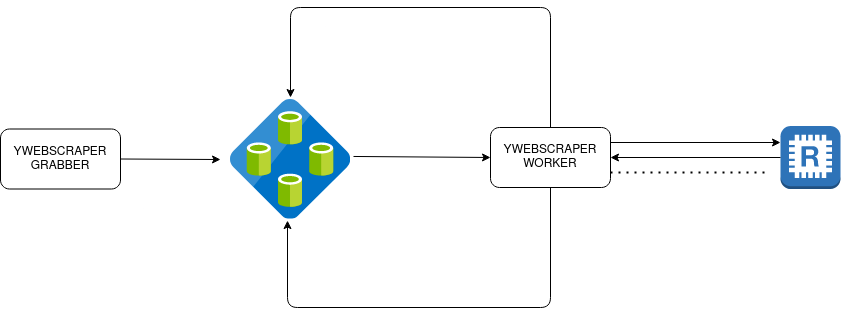
\includegraphics[width=1\columnwidth]{chapter4-project/architettura-gestione-url.png} 
    \caption{Architettura della gestione degli url in dettaglio}
\end{figure}
\newpage{}

\subsubsection{Ricerca nuovi url}
Una delle funzionalità del componente "worker" è l'estrazione degli url dalla coda \emph{Celery} e la loro analisi. Il primo controllo riguarda l'aver già analizzato in precedenza l'url estratto o meno. Se l'url non è presente nella cache di redis allora deve essere analizzato altrimento verrà scartato. Ad inizio analisi l'url viene inserito nella cache redis con un \gls{ttl} impostato dall'analista. Il worker quindi si occuperà di contattare il sito richiesto utilizzando il metodo specificato dall'analista e dal codice sorgente andrà ad estrarre e ripulire la lista di url. 


\subsubsection{Pulizia degli url}
Un url (\href{https://datatracker.ietf.org/doc/html/rfc1808.html#section-2.1}{da RFC 1808, Sezione 2.1}) è composto da \newline
\centerline{<scheme>://<netloc>/<path>;<params>?<query>\#<fragment>}
\newline
\begin{itemize}
	\item \textbf{scheme:} indica il protocollo utilizzato;
	\item \textbf{netloc:} \textit{ne}twork \textit{loc}ation, indica il dominio ed i sottodomini (se presenti), il numero di porta e opzionalmente le credenziali con la seguente sintassi: username:password;
	\item \textbf{path:} contiene informazioni sulla specifica risorsa alla quale accedere;
	\item \textbf{params} campo opzionale contenente informazioni aggiuntive sul path, un esempio possono essere le informazioni aggiuntive da portare da una pagina alla successiva;
	\item \textbf{query} campo opzionale contenente informazioni aggiuntive sul path, come da nome questo campo contiene le query;
	\item \textbf{fragment} campo opzionale contenente informazioni aggiuntive sul path, un esempio possono essere i '\#' che indicano in quale parte della risorsa portare la vista.
\end{itemize}
\noindent
Per realizzare una pulizia degli url completa. serve fare le seguenti operazioni:
\begin{enumerate}
	\item Per evitare di analizzare due pagine identiche con campi fragment differenti, viene eliminato il campo opzionale fragment;
	\item Rendere tutti i caratteri nei campi scheme e netloc minuscoli;
	\item Eliminazione di tutti gli url con contenuto nel campo scheme differente da http o https;
	\item Aggiunta di http nel campo scheme in caso in cui sia vuoto;
	\item Se l'url analizzato è relativo lo si trasforma in url assoluto;
	\item Eliminazione di url uguali all'url iniziale inserito dal modulo "master", all'url precedente e all'url corrente;
	\item Eliminazione degli url presenti nella lista di siti da non esplorare stilata dall'analista.
\end{enumerate}

\subsubsection{Riprovare url}

L'analisi di alcuni url non andrà sempre a buon fine, per questo è stato necessario progettare una logica solida per ritentare il procedimento. Quando l'analisi di un url fallisce per qualsiasi motivo, esso viene reinserito nella coda contenente gli url da analizzare; all'url verrà assegnata una priorità minore, andando quindi ad inserirlo in fondo alla coda. Viene inoltre modificato il \gls{ttl} dell'url nella cache di \emph{Redis}, inserendo un \gls{ttl} minore, in modo che vengano ignorati per un breve lasso di tempo nuovi tentativi con lo stesso url non funzionante, così da non non sovraccaricare il server. Se lo stesso url viene riprovato n volte fallendo, con n scelto dall'analista, allora l'url viene scartato definitivamente.


\subsection{Worker e ricerca di informazioni interessanti}

Il componente denominato "worker" oltre a gestire gli url andrà ad analizzare la pagina alla ricerca di informazioni considerate interessanti.
\begin{figure}[!h] 
    \centering 
    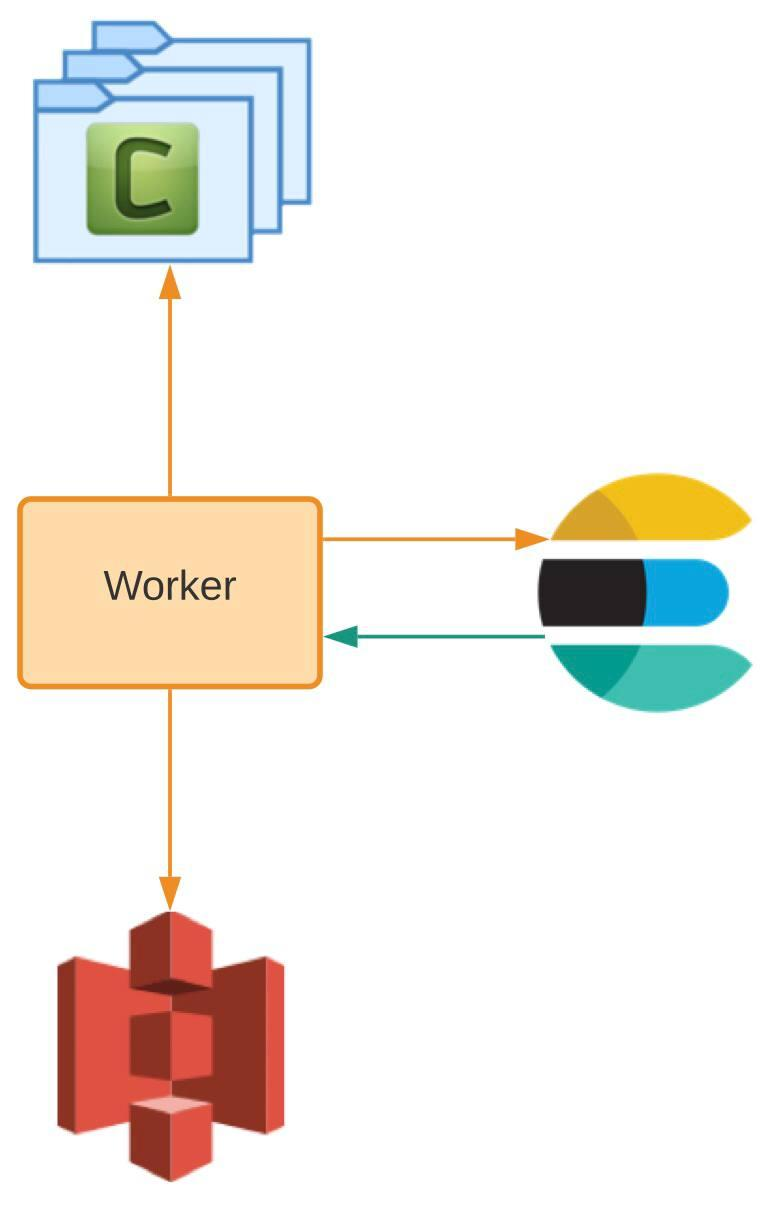
\includegraphics[width=0.4\columnwidth]{chapter4-project/architettura-match-search.png} 
    \caption{Architettura della ricerca di match in dettaglio}
\end{figure}

\subsubsection{Ricerca informazioni interessanti}

La ricerca di informazioni interessanti avviene ricercando occorrenze sulla pagina html, tramite l'utilizzo di molteplici e complesse \emph{regex} stese dall'analista in precedenza. Queste \emph{regex} offrono un grado di granularità aggiuntivo poichè esse vengono sviluppate specificatamente per ogni azienda cliente. Se invece il contenuto del sito non è analizzabile, ad esempio un'immagine, allora viene analizzato l'\emph{header} restituito dal server. Quando vengono trovate occorrenze in un url si crea l'\emph{hash} della pagina tramite un algoritmo e viene controllato se l'\emph{hash} è presente su elasticsearch. Se non è presente allora viene mandato il sito con diverse informazioni aggiuntive nella coda \emph{Celery}. La coda è per un modulo differente presente nella infrastruttura, da questa coda infatti le informazioni vengono elaborate e se ritenute valide aggiunte ad \emph{Elasticsearch}. \newline{}
Se l'\emph{hash} non è presente su \emph{Elasticsearch} viene inoltre salvato il codice sorgente ed una istantanea della pagina su un \emph{bucket} di \emph{Amazon S3}.
\section{Risoluzione difficoltà incontrate}

Durante il progetto, sono state individuate e risolte diverse problematiche. Prenderemo in esempio uno dei problemi affrontati in modo da esporre il modus operandi per l'individuazione e risoluzione.
Ad ogni milestone settimanale raggiunta seguiva un periodo di test durante il quale il modulo operava e venivano raccolti diversi dati di diagnostica. Questi dati venivano poi studiati e verificato se risultassero in linea con le aspettative.

\subsection{Individuazione problema}
Durante la terza settimana di stage, avendo correttamente impostato i \emph{log} ed il codice, è stato possibile osservare i risultati delle prime run di test. Questi test hanno riportato dei dati estremamente diversi da quanto previsto. La memoria utilizzata cresceva sempre di più fino ad un arresto anomalo del programma dopo molte iterazioni. Questo tipo di problema viene chiamato "\emph{memory leak}", ovvero della memoria non viene liberata correttamente dal programma e rimane in utilizzo, accumulandosi.

\begin{figure}[!h] 
    \centering 
    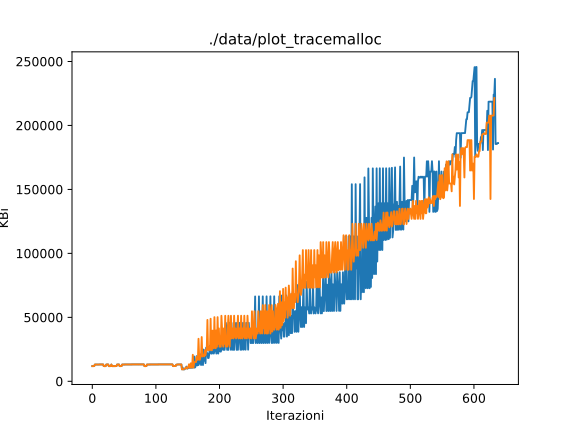
\includegraphics[width=0.8\columnwidth]{chapter4-project/test_con_memory_leak.png} 
    \caption{Test con memory leak}
\end{figure}

\subsection{Risoluzione del memory leak}

Per la risoluzione del problema è stata prima effettuata una analisi del codice scritto, andando a stilare una lista di possibili problematiche collegate alla gestione della memoria. Una prima risoluzione delle problematiche legate al codice, non ha portato a miglioramenti nelle prestazioni. Per questo motivo è stata fatta una ricerca di problemi noti riguardanti le tecnologie utilizzate. Dalla ricerca è risultato che la libreria \emph{Celery}, con alcune specifiche impostazioni, non rilasciasse correttamente la memoria. Cambiando le impostazioni ed eseguendo una nuova run di test, si è potuto osservare come la memoria venisse liberata correttamente.

\begin{figure}[!h] 
    \centering 
    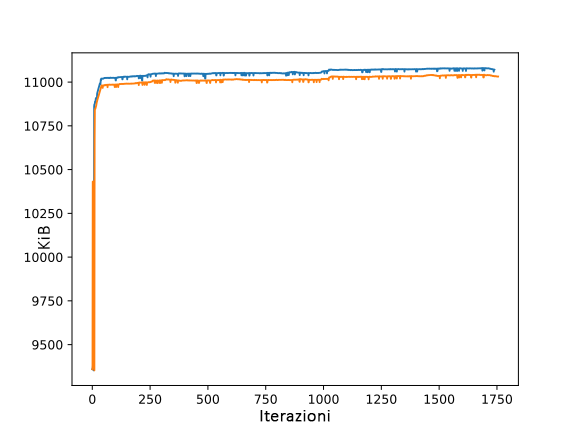
\includegraphics[width=0.8\columnwidth]{chapter4-project/test_senza_memory_leak.png} 
    \caption{Test senza memory leak}
\end{figure}             % Progettazione e sviluppo
% !TEX encoding = UTF-8
% !TEX TS-program = pdflatex
% !TEX root = ../tesi.tex

%**************************************************************
\chapter{Verifica e validazione}
\label{cap:verifica-validazione}
%**************************************************************

\intro{In questo capitolo viene descritto come sono state affrontate le attività di verifica e
validazione del prodotto.}\\

%**************************************************************
\section{Considerazioni}
\label{sec:considerazioni}

Nel piano di lavoro, redatto dal tutor aziendale e approvato dal tutor interno, veniva menzionato lo sviluppo del test automatici come un obiettivo opzionale, preferendo ad essi nuove feature. Per questo, in accordo con il mio tutor aziendale, mi sono dedicato maggiormente all’implementazione e documentazione di esse. Ho comunque avuto modo di effettuare dei test manuali sull’applicativo, verificando il suo corretto funzionamento. I test automatici, che per mancanza di tempo non sono stati sviluppati, verranno implementati successivamente dall’azienda, per provare l’effettiva qualità del software prodotto.

\section{Analisi statica}

Per effettuare l’analisi statica del codice, non sono stati utilizzati particolati strumenti come per esempio linter, questo perché ho ritenuto che l’IDE PyCharm fornisse aiuti più che sufficienti. È noto che PyCharm suggerisce correzioni per eventuali errori introdotti nel codice e miglioramenti durante la scrittura del codice.
In particolare, PyCharm segnala, più comunemente:
\begin{itemize}
	\item incoerenza tra tipi di dati coinvolti in un’istruzione se utilizzati i type hint;
	\item codice non raggiungibile dal flusso di controllo;
	\item variabili dichiarate ma non utilizzate;
	\item metodi dichiarati ma non implementati;
	\item errori di sintassi;
	\item controllo delle librerie importate ma non utilizzate.
\end{itemize}

Inoltre, per concludere, PyCharm offre due funzionalità che ho utilizzato spesso, una è la formattazione automatica del codice e l’altra l’importazione e organizzazione delle classi, sempre automatica.

\section{Analisi dinamica}

Per quanto concerne l’analisi dinamica, nel corso dell’intera fase di codifica, ho potuto verificare il codice utilizzando lo strumento integrato di PyCharm per effettuare il debug, insieme alla libreria Python logger. I test sono stati tutti effettuati manualmente, a questo fine sono state create tre macchine virtuali connesse nella stessa rete. La prima centralizza i servizi utilizzati quali redis e rabbitmq ed inoltre il modulo denominato master, le altre due macchine invece effettuavano lo scraping utilizzando il modulo worker collegandosi ai servizi offerti dalla prima macchina. \newline{}
Al termine di una run di test viene effettuato un lavoro di analisi dei log. Utilizzando una libreria python da me sviluppata si può avere una visualizzazione grafica delle informazioni ritenute interessanti dall'analista, facilitando il lavoro. Un esempio concreto è l'analisi dell'utilizzo di memoria da parte del modulo durante le varie iterazioni, una rappresentazione grafica può risultare più facilmente intepretabile.

\begin{figure}[!h] 
    \centering 
    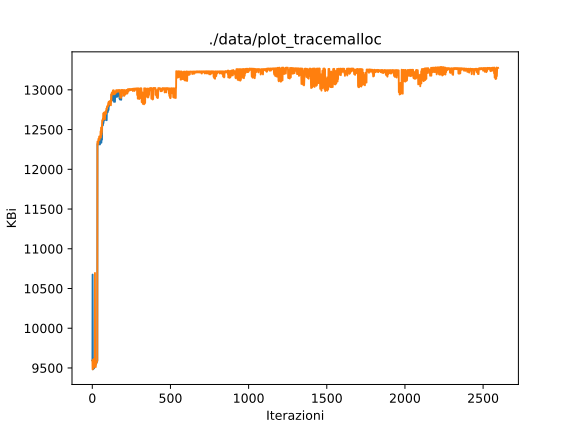
\includegraphics[width=0.6\columnwidth]{chapter5-verify/tracemalloc.png} 
    \caption{Visualizzazione utilizzo memoria}
    \label{fig:visualizzazione-utilizzo-memoria} 
\end{figure}




             % Verifica e validazione
% !TEX encoding = UTF-8
% !TEX TS-program = pdflatex
% !TEX root = ../tesi.tex


%**************************************************************
\chapter{Conclusioni}
\label{cap:conclusioni}
%**************************************************************

%**************************************************************
\section{Raggiungimento degli obiettivi}
La maggior parte degli obiettivi è stata soddisfatta. Gli obiettivi non soddisfatti sono OP06 per scelta dell'azienda e D09 per mancanza di tempo. Gli obiettivi stesi, inizialmente, erano una serie di \emph{feature} desiderate, di cui non era stata fatta una analisi del tempo richiesto. Riuscire dunque a completare la maggioranza dei requisiti ha superato le aspettative iniziali dell'azienda.

%**************************************************************
\section{Conoscenze acquisite}
Questo stage ha contribuito a formarmi in un ambito a me completamente nuovo come quello del dark web e dei web crawler, permettendomi di fare esperienza nel lavoro su strutture complesse, come quella della piattaforma di \emph{Cyber Threat Intelligence} proprietaria. Il progetto, in particolare, mi ha permesso di creare un nuovo modulo che coprisse una area prima non ricercata ed inoltre ha potuto aiutarmi nel rafforzare le mie conoscenze in aree più tecniche nell'ambito dei sistemi operativi, come l'utilizzo di sistemi unix, la configurazione di macchine e la configurazione di reti. A livello aziendale, invece, questo stage ha permesso di dotare la piattaforma aziendale dei mezzi necessari per poter effettuare scraping su buona parte del dark e clear web, indipendentemente dalla struttura del sito. Ciò significa che l’azienda attualmente possiede uno strumento personalizzato ed estendibile per soddisfare le proprie esigenze. \newline{}
Nel mio percorso di stage ho avuto modo di conoscere nuove tecnologie e strumenti, imparando ad apprezzare pregi e difetti di ognuno, per questo è stato fondamentale apprendere rapidamente tecnologie mai utilizzate in precedenza.
Da questa esperienza ho potuto approfondire la mia conoscenza del linguaggio \emph{Python} imparato durante il corso di Ingegneria del Software e le conoscenze di sicurezza informatica imparate nel corso di Cybersecurity, applicandolo allo sviluppo di un applicativo scalabile e performante.
\newpage
%**************************************************************
\section{Valutazione personale}

Considero l'esperienza di stage nel complesso positiva. Quasi tutti gli obiettivi sono stati portati a termine ed il modulo realizzato è funzionante ed operativo oltre che facilmente estensibile. In azienda mi è stata data la possibilità di svolgere il tirocinio in modalità duale, scegliendo autonomamente i giorni in cui lavorare in presenza e quelli in cui lavorare da remoto. Il progetto è stato seguito dal tutor aziendale Matteo Neri, che si è sempre dimostrato aperto al confronto e a lasciarmi autonomia decisionale quando possibile. \newline{}
Fin dal primo giorno di sviluppo ero sicuro che sarei riuscito a completare il progetto in maniera soddisfacente nei tempi richiesti e così è stato, imprevisti e problematiche non sono mancati ma sono sempre stati risolti.
             % Conclusioni
\appendix                               
%\input{capitoli/capitolo-A}             % Appendice A

%**************************************************************
% Materiale finale
%**************************************************************
\backmatter
\printglossaries
\input{inizio-fine/bibliografia}
\end{document}
